\documentclass{article}
% \usepackage[utf8]{inputenc}

% usage: from Options > configure TexStudio > Build > add user command
% makeindex -s nomencl.ist -t %.nlg -o %.nls %.nlo
% Now run pdflatex -> Make Nomenclature -> pdflatex
\usepackage{nomencl}
\makenomenclature

\usepackage{tikz}
\usetikzlibrary{automata,positioning, shapes.geometric}
\usepackage{subfig}
\usepackage{pgf}
\usepackage{float}
\usepackage{titlesec}
\usepackage[nottoc]{tocbibind}
\usepackage{amsmath}
\usepackage{hyperref}
\usepackage{enumitem}
\usepackage{listings}
\usepackage{xcolor}
\usepackage{amsmath,amssymb,amsthm}
\usepackage{graphicx}
\graphicspath{./images/}



% set builder notation utility function, usage: \Set{ x\in A \given x^2 \geq 3 }
\usepackage{mathtools}
\newcommand\SetSymbol[1][]{\nonscript\:#1\vert\allowbreak\nonscript\:\mathopen{}}
\providecommand\given{} % to make it exist
\DeclarePairedDelimiterX\Set[1]\{\}{\renewcommand\given{\SetSymbol[\delimsize]}#1}

% some stuff for C++
\lstset { %
	language=C++,
	backgroundcolor=\color{black!5}, % set backgroundcolor
	basicstyle=\footnotesize,% basic font setting
	breaklines=true,
	postbreak=\mbox{\textcolor{red}{$\hookrightarrow$}\space},
	frame=single,
	columns=fullflexible
}

% TABLE OF CONTENTS, MANUALLY SET NESTING DEPTH
%\setcounter{tocdepth}{1} % show sections
%\setcounter{tocdepth}{2} % show subsections
%\setcounter{tocdepth}{3} % show subsubsections
%\setcounter{tocdepth}{4} % show paragraphs
%\setcounter{tocdepth}{5} % show subparagraphs

% VARIABLES
% --- Hide title page
%\newif\ifhidetitle
%\hidetitletrue

% --- make subsections have lettering (e.g. 1.a, 1.b)
% \renewcommand{\thesubsection}{\thesection.\alph{subsection}}

% --- make subsections have arabic numbering (e.g. 1.1, 1.2, ...)
\renewcommand{\thesubsection}{\arabic{subsection}}

% --- End of proof black square (remove if you want default hollow white square)
\renewcommand{\qedsymbol}{$\blacksquare$}

\titlespacing*{\section}
{0pt}{5.5ex plus 1ex minus .2ex}{4.3ex plus .2ex}
\titlespacing*{\subsection}
{0pt}{5.5ex plus 1ex minus .2ex}{4.3ex plus .2ex}


\begin{document}

% --- title, author, date all on title page, use \\ within a {} to linebreak
\title{CPSC 3630\\Assignment 3}
\author{Cody Barnson\\ ID: 001172313}
\date{Nov 10 2018}

% TITLE PAGE, example of variable usage
%\ifhidetitle
%\else

% --- no page numbers for title page and table of contents
\pagenumbering{gobble}
\maketitle
\newpage

% --- uncomment to show the table of contents
%\tableofcontents
%\listoftables
%\listoffigures
\newpage

% --- this 'fi' belongs to the \ifhidetitle \else block above
%\fi

% --- normal page numbers starting from here, can also do roman
\renewcommand{\thesubsubsection}{\thesubsection.\alph{subsubsection}}
\pagenumbering{arabic}


% ====== START HERE

\section*{}

%Prove that for any languageL2, ifL1is regular then the quotientL1/L2is also regular by using a construction similar to the proof of Theorem1.47
\subsection{Prove that for any language $L_2$, if $L_1$ is regular, then the quotient $L_1/L_2$ is also regular by using a construction similar to the proof of Theorem 1.47.}

Let $L_1$ and $L_2$ be 2 languages over the alphabet $\Sigma$.  The quotient of $L_1$ and $L_2$ is the language $L_1/L_2 = \Set{x \given \exists y \in L_2, xy \in L_1}$.  We wish to prove that for any language $L_2$, if $L_1$ is regular, then the quotient $L_1/L_2$ is also regular. \\

Suppose the $L_1$ is regular, then there exists a DFA $M = (Q, \Sigma, \delta, q_0, F)$ that recognizes $L_1$.  We construct the DFA $M' = (Q, \Sigma, \delta, q_0, F')$ to recognize the quotient $L_1/L_2$, where the set of states, $Q$, is the same as in $M$; the alphabet $\Sigma$ is the same; the transition function is the same; the start state $q_0$ is the start state of $M$, and the set of accept states is given by $F' = \Set{q \given \delta(q, a) \in F}$, for each $a \in \Sigma$.  \\

Since for any input, say $x \in \Sigma^*$, that results in accept state $q_{accept} \in F'$, we have $xy \in L_1$, since reading $x$ transitions to accept state in $F'$, and the following $y$ transitions to accept state in the original machine's set of accept states of $F$.  Thus $L_1/L_2$ is regular, whenever $L_1$ is regular.

\subsection{Use the pumping lemma to show that the following language is not regular.}

\begin{equation*}
	A = \Set{w \in \Set{0,1}^* \given \text{the length of $w$ is a perfect square}}
\end{equation*}

Suppose language $A$ is regular.  Then there exists pumping length $n$.  If we consider the string $0^{n^2}$, where $|w| > n$ and $w \in A$ (by definition).  Note, we choose the string of 0 symbols for simplicity, but without loss of generality for this proof (since there is no restriction on $w$ other than its length is a perfect square). For any decomposition $w = xyz$, we have $|y| \geq 1$ and $|xy| \leq n$, so $1 \leq |y| \leq n$.  \\

We can pump $w$ to get $w_1 = xy^2z$, with $n^2 \leq |xy^2z| \leq n^2 + n$.  We notice that the next perfect square has length $(n + 1)^2 = n^2 + 2n + 1$, however since we have the following inequality:

\begin{align*}
	n^2 + n & < n^2 + 2n + 1 \\
	n       & < 2n + 1       \\
\end{align*}

And we only added at most $n$, but need $2n + 1$ added, then $w_1$ must not be a perfect square, and thus $w_1 \not \in A$.  \\

Now, since all possible pumping of $w$ must be in language $A$ if $A$ is regular (by definition), and we have just shown that $w_1 \not \in A$, we have a contradiction, so $A$ must not be regular.

\subsection{Identify and explain clearly the error in the purported proof below that the language described by the regular expression (r.e.)  $0^*1^*$ is not a regular language.}

The proof error is in the following statement: "However $s$ cannot be pumped since the language $\Set{0^n1^n \given n \geq 0}$ is not regular."  \\

Let $L$ be the language in question.  The string $s$, (i.e. $s = 0^p1^p$) has the same number of 0's as 1's, and $0^p1^p \in L$.  If $0^p1^p$ is pumped, it no longer has equal number of 0's and 1's, however the resulting string is still in $L$ because all the 0's come before all 1's.  So $s$ can be pumped, which the proof claims otherwise.  A correct proof would need to choose string $s$ such that $s$ can not be pumped, in order to show that $0^*1^*$ is not regular.


\subsection{Let $B_n = \Set{a^k \given k \text{is a multiple of $n$}}$ where $\Sigma = \Set{a}$.  Prove that for each $n \geq 1$, the language $B_n$ is regular.}

For any $n \geq 1$, $B_n$ is the language consisting of strings $a^{nt}$, where $t < \mathbb{Z}_{\geq 0}$, and for $t = 0$, we have $\epsilon \in B_n, \forall n \geq 1$.  If $B_n$ can be described by some DFA for some fixed $n \geq 1$ then $B_n$ is regular.  We will give such DFA, $M$, that recognizes $B_n$, as depicted below for fixed $n$:

\begin{figure}[H]
	\centering
	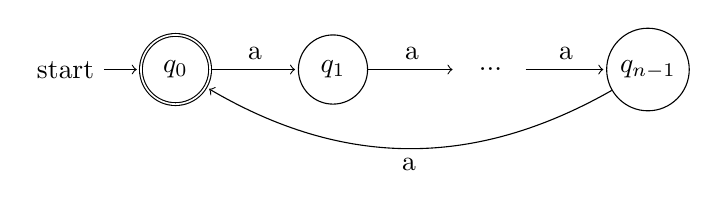
\begin{tikzpicture}[->,shorten >= 1pt,node distance=2cm,on grid,auto]
		\node[state,initial,accepting] (q_0) {$q_0$};
		\node[state] (q_1) [right=of q_0] {$q_1$};
		\node[state,initial text=,color=white,text=black] (q_2) [right=of q_1] {$...$};
		\node[state] (q_3) [right=of q_2] {$q_{n-1}$};
		\path 	(q_0) edge node {a} (q_1)
		(q_1) edge node {a} (q_2)
		(q_2) edge node {a} (q_3)
		(q_3) edge [bend left] node {a} (q_0)
		;
	\end{tikzpicture}
	\caption{State diagram of DFA $M$ that recognizes $B_n$ for some fixed $n \geq 1$.}
\end{figure}

Thus, $B_n$ is regular.

\subsection{Give context-free grammars for each of the following languages where $\Sigma = \Set{0,1}$.}

\paragraph{Note: for each of the following CFG's, assume the start non-terminal is $S$.}

\subsubsection{$\Set{w \given \text{$w$ contains an odd number of symbols}}$}

For this language, we have CFG:

\begin{align*}
	S &\longrightarrow S_0 \;|\; S_1 \\
	S_0 &\longrightarrow 0S_1 \;|\; 1S_1 \\
	S_1 &\longrightarrow 00S_1 \;|\; 01S_1 \;|\; 10S_1 \;|\; 11S_1 \;|\; \epsilon \\
\end{align*}

\subsubsection{$\Set{w \given \text{$w$ contains more 1's than 0's}}$}

For this language, we have CFG:

\begin{align*}
	S &\longrightarrow TS \;|\; 1S \;|\; 1T \\
	T &\longrightarrow TT \;|\; 0T1 \;|\; 1T0 \;|\; \epsilon \\
\end{align*}

\subsubsection{The empty set.}

For this language, we have CFG:

\begin{align*}
	S &\longrightarrow S \\
\end{align*}

Notice that $S$ never resolves, so we get the $\emptyset$.


\subsection{Convert the following CFG where $\Sigma = \Set{0}$ and $A$ is the start non-terminal, into an equivalent Chomsky normal form using the procedure given in Theorem 2.9.}

\subsection{Show that the class of context-free languages is closed under the regular operations: union and star.}

\subsection{Construct a PDA that recognizes the language $\Set{ww^R \given w \in \Set{a,b}^*}$, where $w^R$ is the string $w$ written backwards.}

\end{document}
